%%
%% main.tex - Memoria de la tesis
%%
%%   Copyright 2009-2010 Jesús Torres <jmtorres@ull.es>
%%
%% Esta obra está bajo licencia Creative Commons Reconocimiento 3.0 Unported
%%
\documentclass[b5paper,twoside,11pt,DIV=calc]{scrbook}
\KOMAoptions{open=right,cleardoublepage=empty,headings=big,headsepline=true,
  chapterprefix,bibliography=totoc,captions=tableheading,numbers=enddot,
  draft=false}
\addtocounter{tocdepth}{-1} % No mostrar las subsecciones en las TOC

% Idioma
% http://www.tex-tipografia.com/spanish2.html
% \usepackage[spanish,es-noenumerate,es-tabla]{babel}
\usepackage[british,UKenglish,USenglish,english,american]{babel}
\selectlanguage{english}
\usepackage{ucs}
\usepackage[utf8x]{inputenc}
\usepackage[T1]{fontenc}

\usepackage{float}

% \renewcommand*{\USenglishcontentsname}{\'Indice}

% Fuentes
\usepackage{mathpazo} % Texto con "Palatino" + fuente matemática "Pazo"
\renewcommand{\sfdefault}{uop} % "Optima" como fuente sans serif
\setkomafont{pagehead}{\sffamily\small}
\setkomafont{pagenumber}{\usekomafont{pagehead}}
\setkomafont{caption}{\sffamily\small}
\addtokomafont{captionlabel}{\bfseries}

% Interlineado
\usepackage{setspace}
\onehalfspacing

\recalctypearea % Recalcular las áreas de los bloques de texto
% \usepackage[a4,center,frame]{crop} % Marcas de corte
% \usepackage{showframe} % Marcar los márgenes

% Espacio anterior y posterior al título de cada capítulo
\renewcommand*{\chapterheadstartvskip}{\vspace*{4.50\baselineskip}}
\addtokomafont{chapter}{\fontsize{26}{26}\selectfont}
%\renewcommand*{\chapterheadendvskip}{\vspace{2.25\baselineskip}}

% Listas
% \spanishsignitems

% Notas al pié
\usepackage[multiple]{footmisc}
\deffootnote{1.25em}{1.75em}{\textsuperscript{\thefootnotemark}}

% Separador del título de figuras y tablas
\renewcommand*{\figureformat}{\figurename~\thefigure}
\renewcommand*{\tableformat}{\tablename~\thetable}
\renewcommand*{\captionformat}{\autodot\enskip}
\setcapindent{0em}

% Comments
\newcount\Comments  % 0 suppresses notes to selves in text
\Comments=1   % TODO: set to 0 for final version
\usepackage{color}
% \definecolor{darkgreen}{rgb}{0,0.5,0}
% \definecolor{purple}{rgb}{1,0,1}
% \kibitz{color}{comment} inserts a colored comment in the text
\newcommand{\kibitz}[2]{\ifnum\Comments=1\textcolor{#1}{#2}\fi}
% add yourself here:
% \newcommand{\comment}[2]{\kibitz{red}      {[#1: #2]}}
\newcommand{\comment}[1]{\kibitz{red}      {[COMMENT: #1]}}
\newcommand{\todo}[1]{\kibitz{blue}      {[TODO: #1]}}
\newcommand{\notsure}[1]{\kibitz{green}      {[ELIMINAR?: #1]}}

% Subfiguras
% \usepackage[caption=false, % Usar los captions de KOMA-script
%             labelformat=simple]{subfig}
% \renewcommand\thesubfigure{(\alph{subfigure})} % Paréntesis en las subfiguras
% \renewcommand\thesubtable{(\alph{subtable})} % Paréntesis en las subtablas

\usepackage{epsfig}
\usepackage{tabularx}
\usepackage{graphicx}
\usepackage{caption}
\usepackage{subcaption}

% Tablas
\usepackage{longtable} % notación
\usepackage{tabularx}
\usepackage{booktabs}
\newcolumntype{C}{>{$}c<{$}}
\newcolumntype{L}{>{$}l<{$}}
\newcolumntype{R}{>{$}r<{$}}
\renewcommand*{\arraystretch}{1.1} % Distancia entre filas

% Comando para ayudar a formatear los nombres de los programas
\usepackage{xspace}
\newcommand*{\program}[1]{{\ttfamily #1}}
\newcommand{\Blender}{\program{Blender}\xspace}
\newcommand{\Matlab}{\program{MATLAB}\xspace}
\newcommand{\Makehuman}{\program{MakeHuman}\xspace}

% Listados de código
\usepackage{listings}
\lstset{basicstyle=\small}
\newcommand*{\lstCppMakeShortInline}[1]
  {\lstMakeShortInline[language=C++,basicstyle=\normalsize\ttfamily]#1}
\newcommand*{\lstMatlabMakeShortInline}[1]
  {\lstMakeShortInline[language=MATLAB,basicstyle=\normalsize\ttfamily]#1}
\newcommand*{\lstPythonMakeShortInline}[1]
  {\lstMakeShortInline[language=Python,basicstyle=\normalsize\ttfamily]#1}

% Algoritmos
\usepackage{algorithmic}
\usepackage{algorithm}

% Gráficos
\usepackage{tikz}
\usepackage{graphicx}
\newlength{\figuresheight}
\setlength{\figuresheight}{7cm}
\setkeys{Gin}{totalheight=\figuresheight,keepaspectratio=true}
\graphicspath{{./images/bmps/}{./images/vects/}{./images/}}
\usepackage{ifpdf}
\ifpdf
  \DeclareGraphicsExtensions{.pdf,.mps,.png,.jpg}
\else
  \DeclareGraphicsExtensions{.eps,.mps}
\fi

% Bibliografía
% Citas ordenadas en el orden en que aparecen en la bibliografía (sort).
% % En la primera cita aparecen los nombres de todos los autores (longnamesfirst)
% % \usepackage[longnamesfirst,sort]{natbib}
\usepackage[sort]{natbib}
\bibliographystyle{abbrvnat}
\bibpunct{(}{)}{;}{a}{,}{,}
\setbibpreamble{References shown next are presented in alphabetic order by author. 
References with more than one author are ordered based on the first of them.\par\bigskip}

% Referencias
\usepackage[english]{varioref}
\labelformat{enumi}{(#1)}
\labelformat{equation}{(#1)}

\newcommand{\todoref}[1]{\todo{\ref{#1}}}

% PDFTeX
\pdfimageresolution=300
\pdfcompresslevel=9
\pdfadjustspacing=1 % Asegurar la compatibilidad con la salida normal de TeX
\usepackage[
  bookmarksnumbered=true,
  pdfborder={0 0 0},
  pdfdisplaydoctitle=true,
  pdftitle={Obstacle Detection and Planning for Autonomous Vehicles based on Computer Vision Techniques},
  pdfauthor={N\'estor Morales Hern\'andez},
  pdfsubject={Doctoral Thesis},
  pdfkeywords={XXX, please, add, the, keywords}
  ]{hyperref}

% Para las páginas apaisadas
% \usepackage{lscape}
% \usepackage{pdflscape}
\usepackage{rotfloat} % TODO: Páginas apaisadas en el PDF

% Matemáticas
\usepackage{amsmath}
% \unaccentedoperators
\newcommand{\relphantom}[1]{\mathrel{\phantom{#1}}}
\newcommand{\func}[1]{\mathnormal{#1}}
\newcommand{\mat}[1]{\boldsymbol{\mathrm{\MakeUppercase{#1}}}}
\newcommand{\spc}[1]{\mathbb{#1}}
\newcommand{\dist}[1]{\mathcal{#1}}
\renewcommand{\vec}[1]{\boldsymbol{#1}}
\newcommand{\UPSIGMA}{\boldsymbol{\Sigma}}

\usepackage[printonlyused,withpage]{acronym}
\usepackage{local}

%needed for the full-face titlepage
\usepackage{eso-pic}

% Estructura del documento
\begin{document}

\frontmatter
\label{frontpage}\pdfbookmark{Doctoral Thesis}{frontpage}
\titlehead{
\includegraphics[height=1cm]{ull}
  \vskip 1em
  Facultad de F\'isica y Matem\'aticas \\
  Departamento de Ingenier\'ia de Sistemas y Autom\'atica y Arquitectura y Tecnolog\'ia de Computadores.}
\subject{Doctoral Thesis}
\title{Obstacle Detection and Planning for Autonomous Vehicles based on Computer Vision Techniques}
\author{N\'estor Morales Hern\'andez}
\renewcommand{\codirector}{Leopoldo Acosta S\'anchez\\Jonay T. Toledo Carrillo}
\date{2014}
\maketitle

%%
%% certificado.tex - Memoria de la tesis
%%
%%   Copyright 2009-2010 Jesús Torres <jmtorres@ull.es>
%%
%% Esta obra está bajo licencia Creative Commons Reconocimiento 3.0 Unported
%%
\cleardoublepage
\thispagestyle{empty}
\hfill\begin{minipage}[t]{0.85\textwidth}\parindent 3em
D. Leopoldo Acosta Sánchez, Doctor en Física y Catedrático del
Departamento de Ingeniería Informática de la Universidad de La Laguna.

D. Jonay Tomás Toledo Carrillo, Doctor en Informática y Profesor Contratado Doctor del
Departamento de Ingeniería Informática de la Universidad de La Laguna.
\null\vspace{\baselineskip}

CERTIFICAN:

\vspace{\baselineskip}
que D. Néstor Morales Hernández, Ingeniero en Informática, ha realizado bajo nuestra
dirección la presente Tesis, titulada ``Obstacle Detection and Planning for Autonomous Vehicles based on Computer Vision Techniques (Detección de Obstáculos Basada en Visión por Computador y Planificación para Vehículos Autónomos)'', para optar al
grado de Doctor por la Universidad de La Laguna.

\vspace{\baselineskip}
Con esta fecha, autorizo la presentación de la misma.

\vspace{\baselineskip}
\hfill En La Laguna, a 22 de abril de 2014.
\end{minipage}

\vspace{\baselineskip}
\hfill\begin{tabular}{c}
Los Directores, \\\\\\\\
Leopoldo Acosta Sánchez\\\\\\\\
Jonay Tomás Toledo Carrillo
\end{tabular}

%%
%% dedicatoria.tex - Memoria de la tesis
%%
%%   Copyright 2009-2010 Jesús Torres <jmtorres@ull.es>
%%
%% Esta obra está bajo licencia Creative Commons Reconocimiento 3.0 Unported
%%
\cleardoublepage
\thispagestyle{empty}
\null\vskip 1cm
\textit{\raggedleft
  A Uchy.\\
  \vskip 4cm
  A mis padres, Bernardo e Inmaculada,\\*
  y a mi hermana, Esther.\\
}

%%
%% agradecimientos.tex - Memoria de la tesis
%%
%%   Copyright 2009-2010 Jesús Torres <jmtorres@ull.es>
%%
%% Esta obra está bajo licencia Creative Commons Reconocimiento 3.0 Unported
%%
\cleardoublepage
\thispagestyle{empty}
\addsec*{\protect\centering Agradecimientos}
\markboth{Agradecimientos}{}

En primer lugar, me gustaría agradecer a mis directores de Tesis, Dr. D. Leopoldo Acosta Sánchez y Dr. D. Jonay Tomás Toledo Carrillo, la oportunidad de colaborar en este proyecto, sin el cual no podría haber aprendido lo que he aprendido, ver lo que visto, ni hacer lo que entre todos hemos hecho. Y por supuesto, los buenos consejos y el tiempo prestado, que no ha sido poco, especialmente en las últimas semanas de la Tesis.

No puedo quedarme sin dar mi agradecimiento al Dr. D. Jesús Javier Espelosín Ortega, D. Rafael Arnay del Arco y D. Daniel Perea Ström (¡equipo MARANEDA!), y D. Jonatán Felipe, con los que empecé este camino de cabras que parece no terminar nunca. Nadie nos contó que estaba sin asfaltar, pero estuvimos lo suficientemente locos como para seguir. Agradezco el apoyo ofrecido todos estos años, y sobre todo el buen humor, que nunca ha faltado. Igualmente, agradezco al Dr. D. Jesús Miguel Torres Jorge el haber malgastado parte de su valioso tiempo resolviendo infinitas dudas acerca de todo lo que no era capaz de echar a andar por mí mismo. 

Cómo no, al ``equipo cafeína'', por haber llevado la procastinación a niveles desconocidos. Ellos son: Dña Ángela Hernández López, D. Antonio Morell González, D. Ayoze Marrero Ramos, Dña. Elena Santos Hernández, D. Esteban Rodríguez, D. Eusebio Morell González, D. Francisco Fumero Batista, Dr. D. Iván Castilla Rodríguez, D. Javier Hernández Aceituno, Dr. D. Juan Albino Méndez Pérez (a.k.a. Alexis), Dña. Mariana Cairós González, D. Pedro Antonio Toledo Delgado, Dña. Sara González Pérez, Dña. Silvia de León, Dña. Silvia Vera González, D. Yeray Callero de León, y Dña. Kelin Victoria Zúñiga Meneses. Igualmente, al resto del ya extinto Departamento de Ingeniería de Sistemas y Automática y Arquitectura y Tecnología de Computadores (ISAATC): Dra. Dña. Silvia Alayón Miranda, Dra. Dña. Rosa María Aguilar Chinea, D. Ginés Coll Barbuzano, Dr. D. José Ignacio Estévez Damas, Dra. Dña. Carina Soledad González González, Dr. D. Evelio José González González, Dr. D. Alberto Francisco Hamilton Castro, Dr. D. Sergio Elías Hernández Alonso, Dr. D. Graciliano Nicolás Marichal Plasencia, Dr. D. Roberto Luis Marichal Plasencia, D. Juan Julián Merino Rubio, Dr. D. Lorenzo Moreno Ruiz, Dra. Dña. Vanesa Muñoz Cruz, Dr. D. Sid Ahmed Ould Sidha, Dr. D. José Demetrio Piñeiro Vera, D. Héctor Javier Reboso Morales, Dr. D. José Luis Sánchez de la Rosa, Dr. D. José Francisco Sigut Saavedra y Dra. Dña. Marta Sigut Saavedra.

Vorrei ringraziare il Proffesore Sig. Alberto Broggi per l'opportunità di collaborare e imparare in VisLab, e anche Dott. Paolo Zani e Dott. Mirko Felisa per aver accettato di rivedere questa noiosa tesi e il suo incondizionato supporto durante il mio soggiorno a Parma. Inoltre, apprezzo il consiglio e la grande ospitalità dimostrata da Dott. Luca Bombini, Sig. Michele Buzzoni, Sig. Gabriele Camellini, Dott. Pietro Cerri, Sig. Alessandro Coati, Dott. Rean Isabella Fedriga, Sig. Alessandro Giacomazzo, Dott. Paolo Grisleri, Dott. Paolo Medici, Dott. Pier Paolo Porta, Sig. Mario Sabbatelli e Sig. Pietro Versari, che mi hanno fatto sentire a casa. Anche Sig. Moisés Díaz Cabrera, per la compagnia.

I must thank Prof. Luc Van Gool for allowing me staying some months in PSI/VISICS, acquiring the expertise of his group. I would also like to extend the thanks for the help and the good mood to Mr. Roeland De Geest, Mr. Bert Deknuydt, Mr. Vincent De Smet, Mr. Basura Fernando, Mrs. Rosalia Galiazzi Schneider, Mr. Stam Georgoulis, Mr. Amir Ghodrati, Dr. Hakan Bilen, Mr. Xu Jia, Mr. Jan Knopp, Mr. Paul Konijn, Dr. Marco Pedersoli, Dr. Markus Mathias, Mr. Andelo Martinovic, Mr. Wim Moreau, Mr. José Antonio Oramas Mogrovejo, Mr. Konstantinos Rematas, Mr. Gilad Sharir, Dr. Radu Timofte, Dr. David Tingdahl and Dr. Tatiana Tommasi.

He dejado para el final a los que siempre han estado ahí. A Emilio Brito López, por haberme cuidado la piedra y haberme ayudado a encontrar el océano; a Beatriz Santos Hernández, por demostrar que 360 no es divisible por 5; y a Miguel Ángel Yonte Rodríguez, por recordarme que vivimos bajo la amenaza constante de que un asterisco nos caiga sobre la cabeza. No me olvido de Lilia Ana Ramos y sus consejos sobre los efectos secundarios de la amapola, Jessica Luis López y su inapropiada afición al surf carnavalero, o Ettore Gendusa, sin cuya colaboración esta sección de agradecimientos podría haber acabado en desastre. De Zebenzui Álvarez Lugo aprendí a encontrarle el punto a las cosas, y junto a Jorge Martín Afonso busqué todo lo negro.

Un reconocimiento especial a mi familia, quienes siempre han estado ahí apoy- ándome, animándome y, sobre todo, educándome. No puedo ignorar el hecho de que si no fuera por ellos, no podría haber llegado a lo que he llegado, ni podría haber disfrutado de ciertos privilegios de los que me siento muy agradecido. De mi madre, Inmaculada Hernández Gil, heredé el gusto por viajar, descubrir nuevos horizontes y llegar siempre un poco más lejos; de mi padre, Bernardo Morales Trujillo, aprendí el gusto por conocer, por aprender y por hacer bien las cosas. Este reconocimiento también va para mi hermana, Esther Morales Hernández, que aunque haya puesto mar de por medio, siempre será mi experta en series y cultura contemporánea favorita.

El último agradecimiento lo he reservado para la Doctora Esther Sanromá Ramos (Uchy para los amigos), la persona más importante en mi vida, y con la que más me alegro de haberme cruzado. Agradezco sus esfuerzos por convertirme en una persona socialmente aceptable, la tolerancia demostrada ante mis contínuos \emph{festivales del humor} y su paciencia a la hora de hacerme ver diversos errores de cálculo espaciales (1.35\,m y 1.50\,m no son lo mismo), temporales (10 minutos y media hora no son medidas equivalentes) y espectrales (aunque los árboles sean así, el marrón y el verde por lo visto no combinan). Pero sobre todo, agradezco los buenos momentos y la felicidad que ha sido capaz de darme.










\cleardoublepage
\pdfbookmark{\contentsname}{tableofcontents}
\tableofcontents

\cleardoublepage
\pdfbookmark{\listtablename}{listoftables}
\listoftables

\cleardoublepage
\pdfbookmark{\listfigurename}{listoffigures}
\listoffigures

\cleardoublepage
\pdfbookmark{\listalgorithmname}{listofalgorithms}
\listofalgorithms

%%
%%  acronyms.tex - Obstacle Detection and Planning for Autonomous Vehicles based on Computer Vision Techniques
%%
%%  Copyright 2014 Néstor Morales <nestor@isaatc.ull.es>
%% 
%%  Original version: Copyright 2009-2010 Jesús Torres <jmtorres@ull.es>
%%
%%  This work is licensed under a Creative Commons Attribution 4.0 International License.

\cleardoublepage
\chapter*{Acronyms}\label{ch:acronyms}
\pdfbookmark{Acronyms}{acronyms}
\begin{acronym}[acronyms]
  \acro{RNDF}{Road Network Definition File}
  \acro{MSVM}{Multi-class Support Vector Machine}
  \acro{LIDAR}{Light-Detection And Ranging}
  \acro{HMI}{Human-Machine Interface}
  \acro{GPU}{Graphical Processing Unit}
  \acro{GPS}{Global Positioning System}
  \acro{IMU}{Inertial Measurement Unit} 
  \acro{PF}{Particle Filter}
  \acro{LGT}{Lidar Ground Truth}
\end{acronym}

\acrodef{RNDF}[RNDF]{Road Network Definition File}
\acrodef{MSVM}[MSVM]{Multi-class Support Vector Machine}
\acrodef{LIDAR}[LIDAR]{Light-Detection And Ranging}
\acrodef{HMI}[HMI]{Human-Machine Interface}
\acrodef{GPU}[GPU]{Graphical Processing Unit}
\acrodef{GPS}[GPS]{Global Positioning System}
\acrodef{IMU}[IMU]{Inertial Measurement Unit}
\acrodef{PF}[PF]{Particle Filter}
\acrodef{LGT}[LGT]{Lidar Ground Truth}


\input{notation}

\input{introduction}

\mainmatter
%%
%%  chapter01.tex - Obstacle Detection and Planning for Autonomous Vehicles based on Computer Vision Techniques
%%
%%  Copyright 2014 Néstor Morales <nestor@isaatc.ull.es>
%%
%%  This work is licensed under a Creative Commons Attribution 4.0 International License.
%%

\chapter{Problem Statement}\label{ch:chapter01}

\section{Problem Statement}\label{ch:chapter01_01}

Computer Vision environment understanding targeted at enabling autonomous operation of a robotic platform has been widely studied over the years, leading to the creation of some prototype vehicles \cite{Maurer1996,Pomerleau1996,Broggi1999} which demonstrated that negotiating moderately complex and dynamic situations in real time was possible, albeit challenging. However, it was only with the development effort driven by the DARPA Challenges \cite{Buehler2007, Buehler2009} that the technology required to provide reliable operation both in off-road and urban scenarios proved to be within reach.
The vehicles that successfully took part to this series of events had to integrate planning and actuation capabilities with a sensing suite capable of coping with harsh environments, heavy traffic and wide temperature ranges, while keeping functional over extended amounts of time. Most competitors relied on high-end active sensors \cite{Urmson2008, Montemerlo2008, Bacha2008, Kammel2008}, with some notable exceptions \cite{Broggi2006, Broggi2010}. 

As we discover when looking up to the available literature (See next section, \ref{ch:chapter01_02}), there are many methods for the detection and tracking of obstacles in complex environments, like this for which Verdino is intended to be working. In this sense, a very first approach is that inspired on the work by \cite{primdahl2005change},  \cite{diego2011video} or \cite{vallespi2012prior} was developed. This is based on the fact that, in an image, a high percentage of the scene represented usually corresponds to static objects. Based on that, it looks quite straightforward to think that, having an image representing an area without obstacles, it is possible to detect the obstacles in an scene by just comparing it with an image being taken in real time. For that, we obtained a dataset with geo-referenced images from a closed urbanization taken at different times of the day. A description of this database, as well as of the algorithm pipeline used for the comparison between images pairs can be found at section \todo{ \ref{XXX} }.

However, such approach suffers from several drawbacks. First, as we just use one image per frame, we are no able to know the exact position of the obstacle in the real world \comment{(Anyway, we think that the output of the algorithm is a good starting point for a classification method)}. Also, the quality of detection is highly tied to the size of the image database, so in big areas we need a huge dataset, with the related space and throughput problems associated to that. If we consider changes due to weather or light conditions, this dataset grows exponentially. Finally, we don't know the direction where an obstacle is going to. These are challenging problems that have been solved using different approaches, until we reached a final solution, described in section \todo { \ref{XXX} }.

To solve that, we first developed a method that tries to isolate just the tracking problem with the use of static monocular cameras. Instead of registering pairs of images, we segment the image with the use of foreground extraction techniques, distinguishing between background and foreground. Using the silhouette of the objects in the foreground (which are mainly non-rigid objects, like pedestrians or animals), we apply a non-rigid point set registration algorithm in order to track the different parts of the body of the obstacles separately. This method, inspired in works like those by \cite{starck2007surface}, or \cite{letouzey2011scene}, can be also used for the completion of the global map of the vehicle, or even for tasks more related to \acf{HMI}. This approach is extensively described in section \todo{ \ref{XXX}}.

However, this method still makes use of a very rudimentary method for the localization of the obstacles (See section \todo{ \ref{XXX-subsection_localization}}), and it is limited to static cameras. For the application proposed, we need the cameras installed on the top of the moving prototype, so we can not use foreground segmentation methods anymore for the detection of the objects in the road. A simple solution for that is stop using monocular vision, and start using stereo vision. In the last years, a high number of advanced algorithms has become viable for autonomous driving applications. The problem is that performing a quantitative and meaningful comparison of their performance level, however, is not an easy task, mainly because of the difficulty of producing ground truth information. Older datasets are small, and either synthetic or taken in controlled environments (\cite{Scharstein2002}), thus effectively limiting their usefulness as indicators of the actual algorithms ability to cope with outdoor scenarios. Due to that, it is needed to compare the performance level of some state-of-the-art stereovision-based 3D mapping algorithms in automotive scenarios. This evaluation methodology and the associated results is shown in section \todo{ \ref{XXX}}. \comment{PREGUNTAR A LA GENTE DEL VISLAB SI ESTA DE ACUERDO CON QUE USE ESTO EN LA TESIS, POR SI LAS MOSCAS}.

\comment{Este párrafo y la sección asociada dependerá de lo que consiga sacar más adelante.}\notsure{
Apart from the full-dense 3D reconstruction methods, we also explore the possibility of using a simpler (and faster) reconstruction based on Stixels, like that described by \cite{badino2009stixel}. In particular, we decided to use the implementation by \cite{benenson2012pedestrian}, due to its fast response (about 100 frames per second). The method, described in section \todo{\ref{XXX}}, compares the stixels obtained between frames and tracks the obstacles along the time. This solves all the problems we had: we can use moving cameras, we can locate the obstacles in the map, and also we are able to know the path followed by them.}

Another approach, which makes use of the dense stereo reconstruction algorithms for which we did the evaluation described above, is inspired in the work by \cite{danescu2010particle}, but also from the voxelized world described in \cite{broggi2013}. The key idea is to simplify the 3d reconstructed world into a grid of voxels, each of these representing a certain volume in the world. In this voxelized world, for each voxel above a given occupancy probability threshold, a set of particles part of a particle filter is assigned. Each particle will have a double function: the first, denoting hypotheses (as in the classical particle filter methods); the second, to be used as segmentation criteria in the segmentation of the world into different obstacles. In this way, we consider that two contiguous voxels belong to different obstacles if their obtained direction and sense diverges. A more detailed explanation of the method is found in \todo{\ref{XXX}}.

At this point, we have an acceptable reconstruction of the surroundings of the vehicle, which includes the localization and tracking of the obstacles in the neighborhood of the cart. But the reconstruction of the environment is not the only challenge that an autonomous vehicle has to deal with. Once that a vehicle has an idea of where it is, and where it wants to go, it also needs to know the best way to reach there and, more important, how to avoid the harmful elements it has previously detected using the methods described. This allows a safe trip, both for the pedestrians, cars, etc. in the road, and for the vehicle itself.
As said, Verdino is intended to travel in pedestrian areas where most of the obstacles are pedestrians, so its behavior must be mainly reactive in order to give priority to the safety of paths against the efficiency of the route. Also, there is not a clear traveling path, like a road. Instead of that, the vehicle will be moving around an unstructured area, so there is not something like a \acf{RNDF} that allows a fast calculation of the paths that the car will use to reach a certain point. Because of that, we must consider two different planning levels:
\begin{itemize}
 \item \textbf{Global Planning:}
 As it is not possible to determine a global trajectory based on a \acs{RNDF}, we must use a method able to deal with changing environments for the calculation of a fast and safe path. The idea is that, having a map of the static obstacles in the environment and with the vehicle properly localized on it \cite{Perea2013mcl}, it will generate a path that will allow reaching this destination as fast as possible. This task, which can be solved easily in static environments using graphs or other similar optimization methods, becomes a little bit more challenging in environments like, for example, a parking lot, in which cars are parking and driving off continuously.
 In section \todo{ \ref{XXX} }, the way in which we solved this problem is described. It is based on the border between classes, which is obtained after training a \acf{MSVM} (See Appendix \todo {\ref{XXX}} for more information), considering each single obstacle as a separate class. Instead of using this border for classification purposes, as it is usual, we take advantage of the fact that it will be the safest and smoother distance to the obstacles. Taking this into account, it makes sense to apply this separation line as our path. Also, the use of a different class for each obstacle allows ensuring that the path is safe enough, even in complicate scenarios, like in pedestrian areas.
 
 \item \textbf{Local Planning:}
 In a lower level, we also need a way to make the vehicle know how to follow the generated path. This problem requires a system able to, several times per second, calculate the best steering angle and speed in order to follow the global plan while avoiding the surrounding obstacles. The method, which is inspired in the work of \cite{chu2012local}, receives as input the current position of the vehicle in the map, its orientation, speed and the steering angle. Also, we provide it with the global plan obtained in the upper level. Finally, a map of the dynamic obstacles in the surrounds of the cart is computed and passed to the algorithm.
 
 This dynamic map can be filled with the information provided by sensors like \acp{LIDAR}, among other sensors. But it can can also be computed with the information extracted from cameras, and this is the connection point with the work described in the first part of this Thesis. The detected obstacles are included in the map, so the vehicle is able to avoid them using the calculated steering angle and speed.
 
 The way in which both this map and the speed/steering angle commands is obtained is described in section \ref{XXX}.
\end{itemize}
 
 The whole pipeline of the application developed for this thesis is shown at figure \ref{fig:cp01_pipeline}. 
 
 \begin{figure}[thb]\label{fig:cp01_pipeline}
      \centering
      \includegraphics{pipeline}
      \caption{Pipeline of the modules described in this Thesis.}
\end{figure}

From the images captured in real-time, obstacles are located and passed to the module in charge of the generation of the dynamic costmap. At the same time, the static map is used for the generation of a feasible trajectory. Using the current position and vehicle status, the local planner tries to compute the proper commands in order to follow the global plan while trying to avoid the obstacles included in the dynamic costmap.

\section{Previous Work}\label{ch:chapter01_02}

Research on autonomous vehicles is a task being developed for a long time and for which a big effort has been carried on. A proof of that is the extensive literature existing about that topic, in special since the first of the DARPA Challenges (\cite{Buehler2007, Buehler2009}). Since then, the literature related to the topic has increased. Also, the interest on the use of Computer Vision in autonomous vehicles is growing, due to the possibilities that images offer when compared to other sensors, like \acp{LIDAR}.
In 1996, the ARGO project... \todo{Continuar desde aquí, una vez tenga una especie de historia de los vehiculos autonomos, en la intro.}
\todo{TerraMax, VIAC, Braive, Annieway y cualquier otro que pille por el camino.}
As depicted from section \ref{ch:chapter01_01}, the topics described in this thesis are quite diverse, so it is fair to review the state-of-the art of each of these topics separately.

\subsection{Change detection for obstacle localization in images}\label{ch:chapter01_02_01}

blah blah blah blah blah blah blah blah blah blah blah blah blah blah blah blah blah blah blah blah blah blah blah blah blah blah blah blah blah blah blah blah blah blah blah blah blah blah blah blah blah blah blah blah blah blah blah blah blah blah blah blah blah blah blah blah blah blah blah blah blah blah blah blah blah blah blah blah blah blah blah blah blah blah blah blah blah blah blah blah blah blah blah blah blah blah blah blah blah blah blah blah blah blah blah blah blah blah blah blah blah blah blah blah blah blah blah blah blah blah blah blah blah blah blah blah blah blah blah blah blah blah blah blah blah blah blah blah blah blah blah blah blah blah blah blah blah blah blah blah blah blah blah blah blah blah blah blah blah blah blah blah blah blah blah blah blah blah blah blah blah blah blah blah blah blah blah blah 

\subsection{Non-rigid point set registration for obstacle tracking}\label{ch:chapter01_02_02}

blah blah blah blah blah blah blah blah blah blah blah blah blah blah blah blah blah blah blah blah blah blah blah blah blah blah blah blah blah blah blah blah blah blah blah blah blah blah blah blah blah blah blah blah blah blah blah blah blah blah blah blah blah blah blah blah blah blah blah blah blah blah blah blah blah blah blah blah blah blah blah blah blah blah blah blah blah blah blah blah blah blah blah blah blah blah blah blah blah blah blah blah blah blah blah blah blah blah blah blah blah blah blah blah blah blah blah blah blah blah blah blah blah blah blah blah blah blah blah blah blah blah blah blah blah blah blah blah blah blah blah blah blah blah blah blah blah blah blah blah blah blah blah blah blah blah blah blah blah blah blah blah blah blah blah blah blah blah blah blah blah blah blah blah blah blah blah blah 

\subsection{Evaluation of stereo 3D reconstruction algorithms}\label{ch:chapter01_02_03}

blah blah blah blah blah blah blah blah blah blah blah blah blah blah blah blah blah blah blah blah blah blah blah blah blah blah blah blah blah blah blah blah blah blah blah blah blah blah blah blah blah blah blah blah blah blah blah blah blah blah blah blah blah blah blah blah blah blah blah blah blah blah blah blah blah blah blah blah blah blah blah blah blah blah blah blah blah blah blah blah blah blah blah blah blah blah blah blah blah blah blah blah blah blah blah blah blah blah blah blah blah blah blah blah blah blah blah blah blah blah blah blah blah blah blah blah blah blah blah blah blah blah blah blah blah blah blah blah blah blah blah blah blah blah blah blah blah blah blah blah blah blah blah blah blah blah blah blah blah blah blah blah blah blah blah blah blah blah blah blah blah blah blah blah blah blah blah blah 

\subsection{Stixel World}\label{ch:chapter01_02_04}

blah blah blah blah blah blah blah blah blah blah blah blah blah blah blah blah blah blah blah blah blah blah blah blah blah blah blah blah blah blah blah blah blah blah blah blah blah blah blah blah blah blah blah blah blah blah blah blah blah blah blah blah blah blah blah blah blah blah blah blah blah blah blah blah blah blah blah blah blah blah blah blah blah blah blah blah blah blah blah blah blah blah blah blah blah blah blah blah blah blah blah blah blah blah blah blah blah blah blah blah blah blah blah blah blah blah blah blah blah blah blah blah blah blah blah blah blah blah blah blah blah blah blah blah blah blah blah blah blah blah blah blah blah blah blah blah blah blah blah blah blah blah blah blah blah blah blah blah blah blah blah blah blah blah blah blah blah blah blah blah blah blah blah blah blah blah blah blah 

\subsection{3D object tracking}\label{ch:chapter01_02_05}

By processing the data captured by sensors, it is desired to obtain the position, speed and size of an obstacle. However, usually sensors don't provide this information, so we need to process the information over time and do the tracking of detected obstacles. Many approaches that try to solve this problem, like \cite{danescu2012particle}, assume that obstacles have an standard geometry, and they are modeled as cuboids with associated position, size and speed vectors. This assumption is mostly correct in environments like highways, country roads, and certain urban scenarios, in which almost all the obstacles are cars, trucks or buses which can be simplified as cuboids. Also, these approaches tend to consider a flat ground.
However, this assumption cannot always done, as happens in pedestrian areas, intersections, off-road... In this case, we need to deal with specific shapes, sometimes with concave surfaces. The problem with this kind of obstacles is that methods that assume cuboid-shaped objects tend to wrap the obstacles with a convex shape, which causes an overestimation of their volume (\cite{broggi2013}). Another problem are those objects that are not laying on the ground, as happens with hanged traffic lights, tree crowns, lamps, etc. Usually, they are integrated into an occupancy grid as if they were touching the ground. About the ground plane assumption, in cases like that of an off-road scenario, it is important to estimate the real slope of the road in order to get good results.
Based on how much information they use, we can divide object tracking methods into two subcategories:
\begin{itemize}
 \item \emph{2.5D Solutions:} They do not make use of the complete information provided by 3D points. Instead of that, they tend to use elevation maps composed of uniform size cells. Each cell just stores occupancy and height information. This is the kind of methods that, as described before, usually consider obstacles as being in contact with a flat ground.
 In these methods, tracking is done before the complete reconstruction is done, in an intermediate point based on an specific feature. Based on this intermediate feature, we can distinguishing different kind of approaches:
  \begin{enumerate}
   \item \emph{Use of the 3D point as feature.} An example of this is the so called 6D vision (\cite{franke20056d}), in which the 3D stereo vision extracted information is combined with an efficient implementation of an optical flow in the image space based on a \acf{GPU}. Relevant points are tracked using a Kalman filter.
   \item \emph{Dynamic stixels.} \todo{This approach has been longer discussed in section \ref{ch:chapter01_02_04}.}\comment{Cambiar en caso de que al final no meta los stixels}
   \item \emph{Tracked image features.} As example, check the work by \cite{barth2009estimating}. In this work, obstacles are represented as a rigid 3D point set which are tracked in terms of feature displacements and depth measurements.
   \item \emph{Sensor fusion.} \cite{wu2009collision} reconstruct the objects as cuboids from a stereo point cloud. In this process, position and speed values are improved to a very accurate value by the use of a radar along with stereo.
   \item \emph{Occupancy grids.} This is a very popular choice for tracking. An occupancy grid is a probabilistic map of the driving environment, which encodes the past and present knowledge from sensor data, and which can be updated dynamically when new information is available. These occupancy grids can be cartesian, with rectangular cells, polar, or even a relation between columns in an image an the disparity. An example of this is the method by \cite{danescu2012particle}, which has inspired part of the work described in section \todo { \ref{XXX}}.
   Another advantage of the model based on an occupancy grid is that it makes easier a collaborative update of the grid, which allows the usage of data from several sensors and observers.
  \end{enumerate} 
 \item \emph{3D Solutions:} Usually based on complex grid maps that use complete 3D information. Again, depending on how this grid is represented, we find 
 \begin{enumerate}
   \item \emph{Octree connected cubes.} An example is the work by \cite{wurm2010octomap} or \cite{broggi2013}.
   \item \emph{Adjacent stacks of cells}, as described in \cite{Moravec96robotspatial} 
 \end{enumerate}
\end{itemize}

\subsection{Global planning}\label{ch:chapter01_02_06}

blah blah blah blah blah blah blah blah blah blah blah blah blah blah blah blah blah blah blah blah blah blah blah blah blah blah blah blah blah blah blah blah blah blah blah blah blah blah blah blah blah blah blah blah blah blah blah blah blah blah blah blah blah blah blah blah blah blah blah blah blah blah blah blah blah blah blah blah blah blah blah blah blah blah blah blah blah blah blah blah blah blah blah blah blah blah blah blah blah blah blah blah blah blah blah blah blah blah blah blah blah blah blah blah blah blah blah blah blah blah blah blah blah blah blah blah blah blah blah blah blah blah blah blah blah blah blah blah blah blah blah blah blah blah blah blah blah blah blah blah blah blah blah blah blah blah blah blah blah blah blah blah blah blah blah blah blah blah blah blah blah blah blah blah blah blah blah blah 

\subsection{Local planning}\label{ch:chapter01_02_03}

blah blah blah blah blah blah blah blah blah blah blah blah blah blah blah blah blah blah blah blah blah blah blah blah blah blah blah blah blah blah blah blah blah blah blah blah blah blah blah blah blah blah blah blah blah blah blah blah blah blah blah blah blah blah blah blah blah blah blah blah blah blah blah blah blah blah blah blah blah blah blah blah blah blah blah blah blah blah blah blah blah blah blah blah blah blah blah blah blah blah blah blah blah blah blah blah blah blah blah blah blah blah blah blah blah blah blah blah blah blah blah blah blah blah blah blah blah blah blah blah blah blah blah blah blah blah blah blah blah blah blah blah blah blah blah blah blah blah blah blah blah blah blah blah blah blah blah blah blah blah blah blah blah blah blah blah blah blah blah blah blah blah blah blah blah blah blah blah 

\section{Summary}\label{ch:chapter01_03}

In this chapter, we have described a general idea of the work presented in this Thesis. Also, the pipeline of the final developed application is introduced. All this information will be explained in more detail in the following sections, including implementation details together with some results and a discussion of the advantages/disadvantages of the different methods.


%%
%%  chapter05.tex - Obstacle Detection and Planning for Autonomous Vehicles based on Computer Vision Techniques
%%
%%  Copyright 2014 Néstor Morales <nestor@isaatc.ull.es>
%%
%%  This work is licensed under a Creative Commons Attribution 4.0 International License.
%%

\graphicspath{{./images/chapter05/bmps/}{./images/chapter05/vects/}{./images/chapter05/}}

\chapter{3D object tracking}\label{ch:chapter05}

As we have seen in previous chapters, we still have not solved completely the problem of detection and tracking of the obstacles. Image comparison could be, as said, a good input point for an obstacle classifier, but it is still not able to locate obstacles in the real world with respect to a map o to the vehicle. Also, it is not able to track the obstacles and it is very dependent on the goodness of the database of the area in which the vehicle is driving. Non-rigid point set registration method is not able to detect obstacles using moving cameras. \notsure{Stixels can be a solution, but they do not consider obstacles further from a first plane and they assume a flat road}. 

In this chapter, we will describe a method that, using a point cloud generated from a pair of moving stereo cameras, is able to detect obstacles and model them as a set of voxels. Also, it is able to decide the direction in which objects are moving to. The method described here is inspired in the work by \cite{danescu2012particle}, in the way that a particle filter is used over an occupancy grid in order to detect the obstacles and their directions. However, this method uses a two-dimensional grid. As said in section \ref{ch:chapter01_02_05}, methods based on such a grid are related to which we named as 2.5D methods. The main disadvantages of this kind of methods is that they consider all the obstacles as lying in the ground, and are represented as a convex cuboid that doesn't take into account the complexities of certain obstacles.
As commented in previous sections, Verdino is thought to work in crowded areas, like pedestrian streets or touristic complexes, in which an overestimation of the size of obstacles can lead to an inefficient behavior. So we decided to extend the original method of \cite{danescu2012particle} in order to make it fully three-dimensional, by using a voxelized grid instead of the original cartesian/polar grid, and including some improvements in order to reduce the number of fake positives, among others.

\section{The Method}\label{ch:chapter05_01}

In this method, we generate a voxelized occupancy grid in which the world surrounding the vehicle is divided into a discrete number of voxels of the same size. For each voxel, a occupancy probability is assigned based on the number of points inside the volume represented by it and its neighborhood. Also, during the process, a set of particles will be assigned dynamically during the execution, based on a 3D generalization of the weighting and resampling mechanism described in \cite{isard1998condensation}. These particles will have a double function:
\begin{enumerate}
 \item Denoting hypotheses (as happens with classical particle filters).
 \item Being the building blocks of our world model.
\end{enumerate}

Like this, at each frame, the set of particles obtained in the previous frame (each of these with a certain pose ${(x, y, z)}$ and speed ${(vx, vy, vz)}$) will be evolved using their movement model and assigned to the corresponding voxel, attending to the time that passed between frames and the ego-motion. Then, these particles are re-weighted and resampled.

At this point, particles that passed the resampling process are used to construct the objects that model the environment, joining all these voxels that share a similar orientation and speed. This object reconstruction is done by using a flood fill approach, in a way quite similar to that described in \cite{broggi2013}, but using the vectors of each voxel, instead of color information, as done in their work.

This particle-based approach inherits some advantages from the previous work by \cite{danescu2012particle}:
\begin{itemize}
 \item \emph{It is not necessary to estimate the probability distribution of the speed or the orientation.} These distributions, which in the past have been approximated as histograms (\cite{chen2006dynamic}), Gaussian mixtures (\cite{gindele2009bayesian}) or higher dimensions (\cite{coue2006bayesian}), are not required anymore due to the use the particles. This distribution is obtained directly from the surviving particles of each voxel. 
 \item \emph{Easy encoding of the past and present knowledge from sensor data.} The usage of a voxel grid makes this easier, and allows updating it dynamically when new information is available with a little computational cost.
\end{itemize}

Also, we add some new advantages in our approach:
\begin{itemize}
 \item \emph{Hierarchical object pose, orientation and speed detection.} Object units are detected at lower level as individual voxels, for which we know their individual speed and pose. Joining all these voxels together, we obtain the whole obstacle, whose pose and speed is directly dependent on the voxels which compose it. 
 \item \emph{Fully 3D perception of the object detected.} No previous assumption of the shape of the obstacles is taken, providing an accurate estimation of complex obstacles. The usage of voxels instead of cuboids, allows to have a clear idea of the actual shape of an obstacle, avoiding the overestimation of their real size, which is not acceptable for an application like that described in this Thesis. In this sense, we can have an accurate idea of 3D boundaries of an obstacle or reject it in case it is hanging, like in the case of traffic lights.
 \item \emph{No color information is used.} As we do not use color information coming from the input 3D point cloud, our implementation is ready to accept data from other sensors different from a stereo pair, like \acs{LIDAR}.
 \item \emph{Collaborative update of the grid.} The usage of a voxel grid also allows combining several input sources at the same time. We have not done any work in this sense, but our implementation is ready for such application.
\end{itemize}

The method pipeline is based on six different steps, depicted in figure \todo{ \ref{fig:cp05_pipeline_general} }:
\begin{enumerate}
 \item \emph{3D point cloud generation.} As said before, our implementation is able to work from data coming from any kind of sensor, but in this work, we have been working with stereo cameras. In this step we obtain, from a pair of calibrated images provided by a stereo pair of cameras, a set of 3D points that will be the actual input for our algorithm. At implementation level, this process is done in a separate process, so the point cloud can be used for other tasks in the system. More details of this process are given at section \todo{ \ref{chapter05_01_01} }.
 \item \emph{Ego-motion.} By using images, the orientation and speeds computed for the different objects is biased by the speed of the own vehicle. To avoid this, we need to know our own movement. In section \todo{ \ref{chapter05_01_02} }, this process is better explained.
 \item \emph{Voxelization.} Each of the 3D points obtained in the first step is assigned to a certain voxel. Each voxel has a certain resolution, which covers a parameterized section of the world. In our tests, we have used voxels of a resolution of $(0.25x0.25x0.25)$\,m in the $X$, $Y$ and $Z$ dimensions, respectively, covering a volume going from $-4$\,m to $+4$\,m in the $X$ axis; $0$ to $+24$\,m in the $Y$ axis; and $0$\,m to $3.5$\,m in the $Z$ axis. This process, and how probabilities are assigned to each voxel is explained at section \todo{\ref{chapter05_01_03}}.
 \item \emph{Voxel pose and speed computation.} Based on a \acf{PF} and in the probabilities assigned in the previous step, we calculate the pose and speed of each of the voxels in the grid, as explained in section \todo{\ref{chapter05_01_04}}.
 \item \emph{Object reconstruction.} Once we know the pose and speed of each voxel, and based on a flood fill procedure inspired in the work by \cite{broggi2013} and in the vectors already obtained, similar voxels are assigned to a common final obstacle. For each segmented object, orientation and speed is computed based on the vectors belonging to each of the associated voxels (See section \todo{\ref{chapter05_01_05}}).
 \item \emph{Planning and obstacle avoidance.} Once we know the exact position of the vehicles, and their future movement, we can integrate the results into the rest of the system and use it for the calculation of safe and smooth paths. This process will be described in more depth in the following chapters, in sections \todo{ \ref{chapter05_01_06} }.
\end{enumerate}

\begin{figure}[thb]\label{fig:cp05_pipeline_general}
  \centering
  \includegraphics{pipeline_general}
  \caption{Pipeline of the different steps of the method. \todo{Me olvidé de poner el módulo encargado de filtrar los puntos antes de la fase de voxelizado} }
\end{figure}

In the following sections, all these steps will be explained in a bigger detail.

\subsection{3D point cloud generation}\label{ch:chapter05_01_01}

In this stage, a pair of calibrated images is received and transformed into a disparity map, that will allow us to get the corresponding 3D point cloud. In \todoref{XXX}, we evaluated a set of algorithms, including some pre- and post-processing filters, in order to know which of these is the most suitable for outdoor autonomous navigation applications. From this evaluation, we concluded that best results were given by the configuration we named as \emph{Census-SGM Conf 2}. Unfortunately, we had not access to the optimized version of this configuration at the moment of developing the method explained in this chapter. In the other hand, in the same comparison, we saw that both \emph{BT-SGM} and \emph{ELAS} algorithms had also a good response, and we had an implementation of both of them. The question is: what is the most suitable algorithm for our approach? 

If we look again to the charts in section \todoref{fig:cp05_tfs}, we can notice that the response is similar for both algorithms in the chart at \todoref{XXX-LGT,density,alg}, where the density of all the algorithms is compared for the \acs{LGT} based evaluation. The same happens in the \todoref{XXX-alg,NCC}, despite we concluded that the reliability on this measure is still not clear. In chart \todoref{XXX-alg,NFC} the difference between both algorithms starts becoming bigger, with better results for the \emph{BT-SGM} approach if compared to the \emph{ELAS}. Anyway, results for this last method are not so bad, which is quite better if we attend to the average error computed using the \acs{LGT} (See chart at figure \todoref{XXX,LGT,avg}). This last measure is quite decisive, as too much noise can fake the results. If we look at figure \todoref{XXX-comparacionPointCloudELASvsBTSGM} at section \todoref{XXX-polargridresults}, it is possible to see that the noise generated by \emph{BT-SGM} is much more than that by \emph{ELAS}. This is due to the triangulation-based reconstruction of the disparity map.

Finally, if we look at figure \todoref{XXX-comparacionTiemposELASvsBTSGM} in section \todoref{XXX-polargridresults}, we can see that \emph{ELAS} is much faster than \emph{BT-SGM}, and we require a fast algorithm in order to complete the whole pipeline in real time. \emph{ELAS} is able to work at an average of $17\,Hz$, while \emph{BT-SGM} average is below $5\,Hz$ in the implementation used. Considering this with the fact that the difference between them when looking to other measurements is not so big, we chose to use the \emph{ELAS} algorithm as the base for the point cloud reconstruction.

In figure \ref{fig:cp05_full_filtered_pointcloud}, we can observe the relation between the point cloud generated and the coordinates frame located in the center of the left camera. In this coordinate system, $X$ axis is pointing to the right, $Y$ is the depth of the scene, and $Z$ the height. The rest of frames are explained in more detail in section \todoref{XXX}.

\begin{figure*}[t]
        \centering
        \begin{subfigure}[b]{0.475\textwidth}
                \centering
                \caption{Full Point Cloud}
                \includegraphics[width=\textwidth]{fullPointCloud}\label{fig:cp05_full_pointcloud}
        \end{subfigure}%        
        ~ 
        \begin{subfigure}[b]{0.475\textwidth}
                \centering
                \caption{Filtered Point Cloud}
                \includegraphics[width=\textwidth]{filteredPointCloud}\label{fig:cp05_filtered_pointcloud}                
        \end{subfigure}%
        \caption{Comparison of a point cloud obtained using \emph{ELAS}, before and after the filtering.}\label{fig:cp05_full_filtered_pointcloud}
\end{figure*}

\subsubsection{Point cloud filtering}\label{ch:chapter05_01_01_01}

Once we have obtained the point cloud, we segment the salient volumes by assuming a flat ground. We remove the points below a plane defined by $XY$, as well as those points that are too far from the origin centered at the left camera to fall inside the voxel grid. This distance, and the resolution of each voxel, is parameterized for each dimension, and determines the size of the grid, so

\begin{equation}\label{eq:cp05_filter_limits}
\begin{cases}
W = (I_{max}(X) - I_{min}(X)) / {DX} \\
L = (I_{max}(Y) - I_{min}(Y)) / {DY} \\
H = (I_{max}(Z) - I_{min}(Z)) / {DZ}
\end{cases}
\end{equation}

Here, $W$, $L$ and $H$ are the width, length and height of the voxel grid. $DX$, $DY$ and $DZ$, are the parameterized resolutions of each voxel at dimensions $X$, $Y$ and $Z$, respectively. $I_{max}(d)$ and $I_{max}(d)$ represent the maximal and minimal value of the interval taken in consideration at each dimension $d$. As depicted in the diagram at figure \ref{fig:cp05_intervals}, the left camera is in the center of the grid in the $X$ and $Z$ dimensions, and at the minimal depth in the other dimension.

\begin{figure*}[t]
        \centering
        \includegraphics[width=\textwidth]{intervals}
        \caption{Representation of how the voxel grid is computed. Graphical representation of $\{X, Y, Z\}$, $\{DX, DY, DZ\}$, $\{W, L, H\}$ and $\{(I_{min}(n), I_{max}(n))  | n \in \{X, Y, Z\}\}$ are included, for the sake of clarity.}\label{fig:cp05_intervals}
\end{figure*}

At the end of this process, we will have the filtered point cloud $\mathcal{P}$, which will be the input for the 3D reconstruction stage.

\subsubsection{Using other sensors}\label{ch:chapter05_01_01_02}

Despite we have oriented this work to the usage of a stereo camera as input device, the point cloud generation step and filter step have been implemented as separate processes and, as we will see later, no color information is used. So other sources providing a 3D point cloud stream are acceptable for our algorithm. Also several sensors can provide data simultaneously.

\subsection{Ego-motion}\label{ch:chapter05_01_02}

By using a point cloud referred to the left camera (or a given sensor), speeds and orientations are biased by the movement performed by the ego-vehicle between frames. This movement must be compensated, so we need to know the ego-motion performed by the vehicle. This can be done, in one hand, using the localization method used by Verdino (\cite{Perea2013mcl}), based on the information obtained from an odometric sensor, which combined with the \acf{GPS} signal and an \acf{IMU} device, gives a precise localization Other way to do this is by using a visual odometry system, like that proposed by \cite{geiger2011stereoscan}. \notsure{In section \todoref{XXX}, a comparison of a sensor-based odometric system and a image-based odometry system is performed, concluding that \todo{...} }. As some datasets does not include this odometry information, we have decided to use the visual odometry method in our evaluation tests.

In figure \ref{fig:cp05_tfs}, we can see the different positions at which the vehicle has been located at previous frames, as well as the rest of intermediate coordinate frames used in the application.

\begin{figure}[th]
  \centering
  \includegraphics{tfs}
  \caption{Transformations tree used in our application. \todo{Añadir esquema con los frames arriba a la izquierda de la imagen} }\label{fig:cp05_tfs}
\end{figure}

\subsection{Voxelization}\label{ch:chapter05_01_03}

This is the first stage of the process of the process in charge of the object reconstruction. As said, we have implemented our application in four different processes in order to make it more modular. Three of them have been already described in the previous sections \ref{ch:chapter05_01_01}, \ref{ch:chapter05_01_01_01} and \ref{ch:chapter05_01_02}. This is the fourth.

As input, this process receives the odometry information obtained from the process described in \ref{ch:chapter05_01_02}, and the point cloud $\mathcal{P}$ obtained in section \ref{ch:chapter05_01_01_01}. This point cloud is processed, assigning each point $p_i = (p_x, p_y, p_z), i=1..N_p$ to the corresponding voxel $g_j=(g_w, g_l, g_h), j=1..N_g$, using the expression

\begin{equation}\label{eq:cp05_point_to_voxel}
\begin{cases}
g_w = (p_x - I_{min}(X)) / DX\\
g_l = (p_y - I_{min}(Y)) / DY\\
g_h = (p_z - I_{min}(Z)) / DZ
\end{cases}
\end{equation}

$N_p$ is the number of points in $\mathcal{P}$, $N_g = W * L * H$ is the total number of voxels in the grid $\mathcal{G}$ and $w$, $l$ and $h$ are the integer coordinates inside the grid at $X$, $Y$ and $Z$ dimensions. The grid is represented in the way that the centroid of the voxel $g_j=(0,0,0)$ is located at position $(I_{min}(X) - (DX/2), I_{min}(Y) - (DY/2), I_{min}(Z) - (DZ/2))$.

On each voxel, we store information related to:
\begin{itemize}
 \item The 3D associated points, assigned with the expression at equation \ref{eq:cp05_point_to_voxel}.
 \item The centroids $c=(c_x, c_y, c_z)$ of each voxel.
 \item Uncertainty of the stereo reconstruction values $\sigma_{x_{grid}}$, $\sigma_{y_{grid}}$ and $\sigma_{z_{grid}}$, which will be explained at section \ref{ch:chapter05_01_03_01}
 \item Weights $\omega_{occupied}$ and $\omega_{free}$, described also in the same section.
 \item Density of 3D points $N_p$.
 \item Main orientation and speed vectors $v=(v_x, v_y, v_z)$ and their associated yaw $\psi$, pitch $\theta$ and magnitude $\|v\|$.
 \item Stored particles $q_i = (x, y, z, v_x, v_y, v_z) \in \mathcal{Q}$, with their associated position $x$, $y$, $z$ and velocities $v_x$, $v_y$ and $v_z$.
 \item Obstacle identifier $o_i \in \mathcal{O}$, referencing the obstacle it belongs to. The process in which this identifier is assigned is described in section \todoref{XXX}.
\end{itemize}

\subsubsection{Conditional Probabilities Calculation}\label{ch:chapter05_01_03_01}

Both posterior and conditional probabilities of the received measurement are obtained a method similar to that described in \cite{isard1998condensation}, for a three-dimensional case, as that we have. Probabilities are directly related to the existence of not of 3D points in each one of the voxels. These probabilities will help us, in the next stages, to weight the particles.

For each voxel, we need to know the conditional probability of the associated measurements, under the occupied or free asumption. For that, we have to take into account the specificities of each sensor. In our case, we have based our tests on a stereo camera. In this kind of sensors, uncertainties grow while depth is bigger. So, we want to compute this uncertainty for the centroid $c=(c_x, c_y, c_z)$ associated to each voxel. Then, the uncertainty of the distance reconstruction is given by:

\begin{equation}\label{eq:cp05_uncertainty_distance_reconstruction}
\sigma_{c_y}={{{c_y}^2 \cdot \sigma_d} \over {b \cdot f}}
\end{equation}

Here, $\sigma_d$ is the error in disparity computation; $b$ is the baseline of the stereo system; and $f$ is the focal distance (in pixels).

Based on equation \ref{eq:cp05_uncertainty_distance_reconstruction}, we can derive the lateral and height positioning error $\sigma_w$ and $\sigma_h$:

\begin{equation}\label{eq:cp05_uncertainty_lateral_and_height_reconstruction}
\begin{align}
\sigma_{c_x}={{{c_x} \cdot \sigma_l} \over {c_y}} \\
\sigma_{c_z}={{{c_z} \cdot \sigma_l} \over {c_y}}
\end{align}
\end{equation}
These errors must be mapped into voxel errors. This is just done by dividing them with the voxel size on each dimension.

\begin{equation}\label{eq:cp05_uncertainty_voxel_errors}
\begin{align}
\sigma_w={{\sigma_{c_x}} \over {DX}} \\
\sigma_l={{\sigma_{c_y}} \over {DY}} \\
\sigma_h={{\sigma_{c_z}} \over {DZ}}
\end{align}
\end{equation}

Based on these errors, the idea is to find an approximation for the conditional probabilities of the measurement voxels under the occupied/free assumption. For that, we count the occupied neighbor voxels in the grid. The distance for which we consider a voxel as neighbor comes from the values of $\sigma_w$, $\sigma_l$ and $\sigma_h$. The total number of occupied neighbors is divided by the total number of voxels explored, obtaining the final value of the conditional probability.

\begin{equation}\label{eq:cp05_conditional_prob}
p(m(w,l,h)|occupied) = {
{\sum \limits_{w'=w-\sigma_w}^{w+\sigma_w} \sum \limits_{l'=l-\sigma_l}^{l+\sigma_l} \sum \limits_{h'=h-\sigma_h}^{h+\sigma_h} O(w',l',h')} 
\over 
{(2 \cdot \sigma_w + 1) \cdot (2 \cdot \sigma_l + 1) \cdot (2 \cdot \sigma_h + 1)}}
\end{equation}

, where

\begin{equation}\label{eq:cp05_occupied}
\begin{align*}
 O(w', l', h') &=
  \begin{cases}
   1        & \text{if } %
   %
   {\exists p(x, y, z) \in \mathcal{P} ~|~ p \text{ belongs to } \mathcal{G}(w', l', h')}%
   \\
   0        & \text{otherwise}
  \end{cases}
\end{align*}
\end{equation}

The conditional probability of the measurement given the “free” assumption is

\begin{equation}\label{eq:cp05_conditional_prob}
p(m(w,l,h)|occupied) = 1 - p(m(w,l,h)|free)
\end{equation}

In figure \ref{fig:cp05_voxelization} the obtained voxels are represented. The occupation probability is represented through the alpha channel of each of them, so the opacity is directly related to this probability, being the most transparent ones those with a low value.

\begin{figure}[th]
  \centering
  \includegraphics{voxelization}
  \caption{Voxelization of a given point cloud. Those voxels with a bigger occupation probability are more opaque.\todo{Poner opacidad en función de la probabilidad} }\label{fig:cp05_voxelization}
\end{figure}

\subsection{Voxel pose and speed computation}\label{ch:chapter05_01_04}

The pipeline of this step is represented in figure \ref{fig:cp05_voxel_pose_speed_computation}. One of the advantages of using a grid of voxels is that most of the computation is performed for each of them separately, making it suitable for a parallel implementation. 

An explanation of the subtasks of this step is given next:

\begin{figure}[th]
  \centering
  \includegraphics{voxelPoseAndSpeedComputation}
  \caption{Pipeline of the voxel pose and speed computation stage.}\label{fig:cp05_voxel_pose_speed_computation}
\end{figure}

\subsubsection{Prediction}\label{ch:chapter05_01_04_01}

In this step, we compute the present particle distribution taking into account each particle motion model and the time that has passed between frames. With this new distribution, data will be ready for the next task. In the method developed by \cite{danescu2012particle}, they updated the particle set in a step quite similar to this one. However, in their work, prediction equations used odometric information in order to compensate the ego-motion. In our approach, we do not perform this compensation. This doesn't means that we do not care about our the bias introduced by the vehicle movement, but this movement will be compensated at the end of the process, once we have the orientation and speed of each obstacle. This come with some avantages:
\begin{itemize}
 \item We do not need to translate and rotate the whole grid between iterations, as it is moving together with the left camera based frame.
 \item We just need to apply the motion equations in order to update the particles set.
\end{itemize}

These advantages allows saving a lot of resources. This is the most computationally expensive of the tasks in the method, which is highly dependent on the parameter $N_g$, that controls the number of particles. If we speed up this step, the system will be able to deal with a larger number of particles, improving the results.

Each of the particles $q_i = (x, y, z, v_x, v_y, v_z) \in \mathcal{Q}$ is updated as follows. First, we need a motion model that allows to transform the particles based on the increment of time $\Delta t$ and the parameters of position and speed of the particle. For this purpose, we introduce the state transition matrix $S$:

\begin{equation}\label{eq:cp05_state_transition_matrix}
S =
\left( \begin{array}{cc}
I_{3\times3} & \Delta t \cdot I_{3\times3} \\
0_{3x3} & I_{3\times3} \end{array} \right)
\end{equation}

We also introduce the matrix $\Delta$, which models the stochastic diffusion caused by the uncertainties in the motion model.

\begin{equation}\label{eq:cp05_state_motion_model_uncertainties}
\Delta =
\left( \begin{array}{cccccc}
\delta x & \delta y & \delta z & \delta v_x & \delta v_y & \delta v_z
\end{array} \right)^T
\end{equation}

Here, $\delta x$, $\delta y$, $\delta z$, $\delta v_x$, $\delta v_y$ and $\delta z$, are randomly drawn from a Gaussian distribution of zero mean and a covariance matrix Q equivalent to the state transition covariance matrix of a Kalman filter.

So, the new position of each particle is given by the expression

\begin{equation}\label{eq:cp05_particle_update}
q_{t + 1} = S \cdot q_{t} + \Delta
\end{equation}

\subsubsection{Weighting and resampling}\label{ch:chapter05_01_04_02}

This step is quite similar to the stage with the same name in the work of \cite{danescu2012particle}, with some minor differences, most of them related to the addition of a new dimension. For optimization reasons, in this stage we also perform the calculation of the main orientation and speed vectors associated to each voxel.

As said before, particles are the base of our system. They are used both as hypotheses and as the building blocks of the different obstacles. From these particles, we are going to calculate the main vectors of each voxel, which will be used in later steps for the reconstruction and segmentation of the final obstacles.

But in this step we are more interested in their role as hypotheses. A particle in a voxel is a hypothesis saying that it is occupied, and that it has the speed equal to the speed of the particle. The more particles in a voxel, the more chances to be occupied. If there are not many particles in the voxel, the hypothesis of the voxel being free is supported. The particles are multiplied or deleted depending on how well the occupied or the free hypotheses of each voxel are supported by the measured data.

This step is composed by two steps: Weighting and Resampling. As said, we also include the main vectors calculation in this section, but it could be easily a separate step which is included here just for optimization reasons.

\paragraph{Main vectors calculation}\label{ch:chapter05_01_04_02_01}

Once the survival particles which fall inside an occupied voxel have been computed, main vectors are obtained. The way in which we do that is through an spherical histogram. The idea, depicted in figure \ref{fig:cp05_spherical_hist}, works at follows:
\begin{itemize}
 \item The possible values of yaw $\psi$ that the voxel can take ($[0\dots2\pi]$) is divided in intervals of size $\Delta\psi$; we do the same for the pitch $\theta$, with intervals of size $\Delta\theta$. In our tests, both $\Delta\psi$ and $\Delta\theta$ are set to $5^{\circ}$.
 \item For each particle, we obtain the corresponding value of $\psi$ and $\theta$, and the corresponding bin is increased in one unit. Each bin stores, also, the average of the speeds related to each particle.
 \item The speed and orientation will be given by the bin with the biggest number of related particles.
 \end{itemize}
 
 After this process, each voxel will know their estimated speed and direction. These must be obtained using just the surviving particles after the prediction process. As weighting and resampling is an stochastic process, results could be biased by wrongly duplicated or eliminated particles. In figure \ref{XXX-segmentation} we can view the main vectors obtained for the surviving voxels after the segmentation process.

\begin{figure}[th]
  \centering
  \includegraphics{sphericalHist}
  \caption{Diagram representing an spherical histogram.}\label{fig:cp05_spherical_hist}
\end{figure}

\paragraph{Weighting}\label{ch:chapter05_01_04_02_02}

The number of particles $N_g$ is assumed to be constant, assuming that the real particles inside a voxel have the occupancy value \emph{true}, while that the absence of real particles is considered as the presence of virtual particles with an occupancy value equal to \emph{false}. Based on this idea, as measurement data does not include speed information (we are using as input pure 3D point clouds), the weight of the particles depends only on the \emph{occupied} hypothesis.

So, for each voxel, we are interested on getting the total posterior probability of being occupied or free. In order to obtain these probabilities, we will need the measurement conditional probabilities (weights) of each voxel and the number of free/occupied hypotheses. The total posterior probabilities are given by:

\begin{equation}\label{eq:cp05_total_posterior_probabilities}
\begin{array}{l}
P_{og}={{\omega_{occupied} \cdot N_{og}} \over {\omega_{occupied} \cdot N_{og} + \omega_{free} \cdot N_{fg}}} \\
P_{fg}={{\omega_{free} \cdot N_{fg}} \over {\omega_{occupied} \cdot N_{og} + \omega_{free} \cdot N_{fg}}}
\end{array}
\end{equation}

In these equations, the values of the weights $\omega_{occupied}$ and $\omega_{free}$ are already calculated during the process described at section \ref{ch:chapter05_01_03_01}, so 

\begin{equation}\label{eq:cp05_occupancy_weights}
\begin{array}{l}
\omega_{occupied} = p(m(w,l,h)|occupied) \\
\omega_{free} = p(m(w,l,h)|free)
\end{array}
\end{equation}

; about $N_{og}$ and $N_{fg}$, they are the number of particles having the \emph{occupied} hypothesis (real number of particles in the voxel), and those having the \emph{free} hypothesis, respectively. As said before, we consider the absence of particles as the presence of a set of virtual particles with the hypothesis \emph{free}:

\begin{equation}\label{eq:cp05_number_of_particles}
\begin{array}{l}
N_{og} = | \{ p_i \in \mathcal{P} | p_i \text{ belongs to voxel } g \} | \\
N_{fg} = N_g - N_{og}
\end{array}
\end{equation}

\paragraph{Resampling}\label{ch:chapter05_01_04_02_03}

After the weighting step is done, we can start with the resampling step. After this, the population of particles will be properly updated, so we can use them for the reconstruction of the obstacles. As we do not take into account the free voxels, just real particles (those with the \emph{occupied} hypothesis) will be considered. For each of these particles, we will decide if they are destroyed or multiplied. After the process of resampling has been completed, each voxel will have the proper number of particles.

In the algorithm \ref{alg:cp05_weighting_resampling}, we describe the resampling process. For the sake of clarity, the point in which weighting and main vectors are computed is indicated.

\begin{algorithm}
\caption{Weighting and Resampling}
\label{alg:cp05_weighting_resampling}
\begin{algorithmic}
\State {\comment{A la persona que me esté revisando esto: échale un ojo al algoritmo correspondiente en \cite{danescu2012particle} (pagina 11). No se si es plagio o adaptacion al caso concreto de los voxels y, en parte, a como llevé el cambio de celda a voxel. En general es el mismo algoritmo, pero uní los dos fors por un tema de optimización: no recorro todas las partículas correspondientes buscando el voxel asociado. En vez de eso, recorro para cada voxel (para el cual ya calculé $f_g$) y hago el resampling sólo en las partículas asociadas. A efectos prácticos es lo mismo, sólo que más eficiente :) }}
\Function{MeasurementBasedUpdate}{$\mathcal{G}$} 
  \For {\textbf{each} voxel $g \in \mathcal{G}$}
    \State \textbf{Main vectors computation}
      \State \indent {$g$.computeMainVectors()}
    \State
    \State \textbf{Weighting}
      \State \indent Compute $N_{og}$ and $P_{og}$
      \State
    \State \textbf{Resampling}
      \State \indent Compute resampled number of particles $N_{rg}$
      \State \indent $N_{rg} \gets P_{og} \cdot N_g$
      \State \indent $f_g \gets {{N_{rg}} \over {N_{og}}}$
    \For {\textbf{each} particle $p$ belonging to $g$}
      \State \Comment { The number of particles will be increased.}
      \If { $f_g > 1$ } 
	\State {$F_n \gets \lfloor f_g\rfloor$} \Comment {Integer part}
	\State {$F_f \gets f_g - \lfloor f_g\rfloor$} \Comment {Fractional part}
	\For {$k = 1$ to $F_n - 1$}
	  \State {$g$.makeCopy($p$)}
	\EndFor
	\State $r \gets \text{random value in the range [0 \ldots 1]}$
	\If {$r < F_f$}
	  \State {$g$.makeCopy($p$)}
	\EndIf
      \State \Comment {$f_g < 1$, the number of particles will be decreased.}
      \Else 
	\State $r \gets \text{random value in the range [0 \ldots 1]}$
	\If {$r > F_g$}
	  \State {$g$.remove($p$)}
	\EndIf
      \EndIf
    \EndFor
  \EndFor
\EndFunction
\end{algorithmic}
\end{algorithm}

The algorithm is almost the same as proposed in \cite{danescu2012particle}. The main difference is that, due to optimization reasons we do not split the whole process into two different loops. To do that, instead of having the set of particles separated from the voxels, each voxel knows exactly where its particles are. In the original algorithm, it is necessary to compute and store the value of $f_g$ for absolutely all the voxels in $\mathcal{G}$. After that, the program iterates over all the particles in $\mathcal{P}$. For each of these particles $p$, we need to know the related voxel and look for the computed value $f_g$. In our approach, we assign each particle to its voxel directly at the \emph{initialization} and \emph{prediction} steps, so we can perform all the weighting and resampling step at once, saving a little bit more computational time again.

The resampling process depends on the value of the ratio between the actual number of particles and the number of resampled particles ($f_g$). Based on this value, we know if the particles will be duplicated ($f_g > 1$) or removed ($f_g < 1$). In figure \ref{fig:cp05_weight_and_resample}, an example where the surviving particles after this step are shown. In this case, pedestrians are moving in the negative direction of $X$ and $Y$ axis, so the most of surviving particles have this trend. These will be used in the next step for the calculation of the main vectors representing the movement of each voxel separately.

\begin{figure}[th]
  \centering
  \includegraphics{weightAndResample}
  \caption{Pipeline of the voxel pose and speed computation stage.}\label{fig:cp05_weight_and_resample}
\end{figure}

After this process is finished, we can proceed to the initialization stage.

\subsubsection{Initialization}\label{ch:chapter05_01_04_03}

In this stage, those voxels without particles initialize a new set of them with a number proportional to the occupancy probability. This situation can be reached for two reasons:
\begin{itemize}
 \item This is the first iteration, so none of the voxels has been initialized already.
 \item After the weighting and resampling process, none of the particles survived.
\end{itemize}

This stage is the first step we perform in the execution on the method, and the last at each iteration. It is in charge of ensuring that the number of particles never become zero. Here, we just check each of the voxels $g \in \mathcal{G}$. If there are not particles in the voxel ($N_p = 0$), or the occupancy probability is bigger than the occupancy threshold $\tau_{o}$ ($\omega_{occupied} > \tau_{o}$), a number of particles equal to $N_p$ is initialized in the voxel.

Given the voxel $g \in \mathcal{G}$, each particle is initialized with the position $(x, y, z) = (g.c_x, g.c_y, g.c_z)$, and a random speed $(v_x, v_y, v_z)$ in the range $[0\dots v_{max}(n)]$, being $v_{max}(n)$ an user defined parameter that determines the maximal speed at each dimension $n \in \{ X, Y, Z\}$ that is expected by each voxel. 

In this implementation, we allow vertical movements controlled by the parameter $v_{max}(Z)$. However, in certain situations like planar grounds this movement is not relevant, so it is better to assign it to $0$, so the particles can restrict their movement to the $XY$ plane.

\subsection{Object reconstruction}\label{ch:chapter05_01_05}

Based on the main vectors obtained for each voxel, we can assume that all the adjacent voxels with a similar direction and speed belong to the same obstacle, or at least to the same group of obstacles (for example, we could find a situation in which a group of people are all of them walking together. We are not concerned about this case because if they are considered as a single obstacle is because they are adjacent and there is no traversable space between them. As they walk in the same direction, in practice we can think on them as a single obstacle).

In this sense, we have developed a method inspired in the color-based clustering described by \cite{broggi2013}. However, in our case, the similarity function is not based on color information because of the reasons explained before, so this similarity function is split into three different similarity functions:

\begin{equation}\label{eq:cp05_similarity_functions}
\begin{array}{l}
f_1(o,g)=\| |\vec{v}|_o - |\vec{v}|_g \|\\
f_2(o,g)=\| \phi_o - \phi_g \|\\
f_3(o,g)=\| \theta_o - \theta_g \|
\end{array}
\end{equation}

, where $|\vec{v}|_o$ and $|\vec{v}|_g$ are the modulus of the speeds obtained for an obstacle $o \in \mathcal{O}$ and for a voxel $g \in \mathcal{G}$, respectively. The same applies for the yaw $\phi_o$ and $\phi_g$, and the pitch $\theta_o$ and $\theta_g$ measurements.

The use of these similarity functions has several advantages. The most direct is that the input cloud of our algorithm can be generated by a sensor different from a stereo pair. We could even combine them, as it has been said before. The employed flood-fill based clustering algorithm is described in the algorithm \ref{alg:cp05_clustering}.

\begin{algorithm}
\caption{Clustering algorithm}
\label{alg:cp05_clustering}
\begin{algorithmic}
\Function{Clustering}{$\mathcal{G}$} 
\State {$\mathcal{G'} \gets \mathcal{G}$} \Comment {$\mathcal{G'}$ is the set of not-checked voxels }
\For {\textbf{each} voxel $g \in \mathcal{G'}$}
  \State {$\mathcal{G'} \gets \mathcal{G'} - g$}
  \State {$o \gets \text{ new object containing }g$}
  \State {$\text{insert } g \text{ in } queue$}
  \While {$queue \ne \emptyset$}
    \State {$g' \gets \text{extract first element from the } queue$}
    \For {\textbf{each} $\{ g'' | g'' \in o\} \in N(g')$}
      \If {$ f_1(o,g) < \tau_{v} \textbf{ and } f_2(o,g) < \tau_{\psi} \textbf{ and } f_3(o,g) < \tau_{\theta} $}
	\State {$\text{insert } g'' \text{ in } o$}
	\State {$\text{insert } g'' \text{ in } queue$}
      \EndIf
    \EndFor
  \EndWhile
  \If {$|o| >= \tau_{min\_voxels\_per\_obstacle} \textbf{ and }$\\ 
  \pushcode\pushcode$~~~~o.sz(Z) >= \tau_{min\_obstacle\_height} \textbf{ and }$\\
  \pushcode\pushcode$~~~~o.min(Z) == I_{min}(Z)$}
      \State {$o \text{.updateVectors()}$}
      \State {$\text{insert } o \text{ in } \mathcal{O}$}
  \EndIf
\EndFor
\EndFunction
\end{algorithmic}
\end{algorithm}

The neighborhood of a voxel $g$ represented by the function $N(g)$, as in \cite{broggi2013}, is performed using the Chebyshev distance. When a new voxel $g''$ is added to an obstacle $o$, the voxel identifier is updated. From the obstacle point of view, we just add the voxel to a list associated to each obstacle. Once an obstacle is about to be added to the final set of obstacles, this list will be used for updating the information related to the obstacle centroid, speed and limits on each dimension (See section \ref{ch:chapter05_01_05_01}).

Before adding an obstacle to the final list of obstacles $\mathcal{O}$, we perform a filtering stage which, for optimization reasons, has been integrated in the segmentation process. This filtering procedure is based in a set of assumptions, related to the expected size of the obstacles and their position regarding to the ground. An obstacle is accepted in the final list if:

\begin{itemize}
 \item It is big enough. That is, if the number of voxels (which is directly proportional to its volume) is over the user-defined parameter $\tau_{min\_voxels\_per\_obstacle}$.
 \item It is tall enough. The minimal height is controlled by the parameter $\tau_{min\_obstacle\_height}$
 \item The obstacle is on the ground. This helps to remove flying obstacles like traffic lights or the top of some trees.
\end{itemize}

\subsubsection{Obstacle vectors computation}\label{ch:chapter05_01_05_01}

Once we have the list of voxels that compose each obstacle, we can use it for the calculation of their speed direction and magnitude. We want also to compensate the motion of our vehicle in order to know their real speed. Let $ego_{vx}$, $ego_{vy}$ and $ego_{vz}$ be the vectors that represent the motion of the vehicle regarding to the left camera coordinates frame. Also, $o_{vx}$, $o_{vy}$ and $o_{vz}$ will be the motion vectors of each obstacle and $g_{vx}$, $g_{vy}$ and $g_{vz}$ those for each of the voxels in the list for that obstacle. Then, the final speed for each obstacle will be obtained by applying:

\begin{equation}\label{eq:cp05_obstacle_vectors_computation}
\begin{cases}
o_{vx} = {{\sum\limits_{g \in \mathcal{G}_o} g_{vx}} \over {|\mathcal{G}_o|}} + ego_{vx}\\
o_{vy} = {{\sum\limits_{g \in \mathcal{G}_o} g_{vy}} \over {|\mathcal{G}_o|}} + ego_{vy}\\
o_{vz} = {{\sum\limits_{g \in \mathcal{G}_o} g_{vz}} \over {|\mathcal{G}_o|}} + ego_{vz}
\end{cases}
\end{equation}

Here, $\mathcal{G}_o$ is the list of voxels associated to the obstacle $o$. In figure \ref{fig:cp05_obstacle_vectors_computation}, we have shown a simulation of which will be the future movement of the obstacles if we consider the obstacle speed computed in this stage.

\begin{figure}[th]
  \centering
  \includegraphics{fakePointCloud}
  \caption{Simulation of the obstacles future movement using the computed vectors.}\label{fig:cp05_obstacle_vectors_computation}
\end{figure}

\subsection{Planning and obstacle avoidance}\label{ch:chapter05_01_06}

\todo{Si me da tiempo, intentar meter el dataset de Daimler y hacer unos test de detection rate un poco mejores, incluyendo velocidades.}
The speed vectors of each obstacle, together with their position and the 3D point cloud stored by the associated voxels will be used by the planner of the vehicle in order to perform an efficient and safe planning. This task, which is the final objective of this thesis, will be described in section \todoref{XXX}. A figure of the output of this method being used for planning tasks is shown at figure \todoref{XXX}, in the same section. Also, a video of the pipeline of the whole method described here is available at \todoref{XXX}.

\section{Results}\label{ch:chapter05_02}

\section{Input point cloud}\label{ch:chapter05_02_01}
% Imagen que compara los resultados con ELAS y con BT-SGM
\begin{figure*}[th]
        \centering
        \begin{subfigure}[b]{0.475\textwidth}
                \centering
                \caption{BT-SGM}
                \includegraphics[width=\textwidth]{btsgm}\label{fig:cp05_bt_sgm}
        \end{subfigure}%        
        ~ 
        \begin{subfigure}[b]{0.475\textwidth}
                \centering
                \caption{ELAS}
                \includegraphics[width=\textwidth]{elas}\label{fig:cp05_elas}                
        \end{subfigure}%
        \caption{Comparison of a resulting point cloud obtained using both \emph{BT-SGM} and \emph{ELAS}.}\label{fig:cp05_comparison_bt_sgm_vs_elas}
\end{figure*}

% Comparacion de tiempos
 \begin{figure}[th]
  \centering
  \includegraphics[trim=50 50 90 60, clip]{timesELAS_OPENCV}
  \caption{Comparison of the required time for each of the stereo reconstruction algorithms.}\label{fig:cp05_times_elas_btsgm}
\end{figure}

\section{Ego-motion}\label{ch:chapter05_02_02}
% Añadir comparativa entre libviso y la odometría real
 \begin{figure}[th]
  \centering
  \includegraphics[trim=50 50 90 60, clip]{yaw}
  \caption{Comparison between the yaw values obtained through visual odometry compared to mechanical odometry.}\label{fig:cp05_ego_yaw}
\end{figure}

\begin{figure}[th]
  \centering
  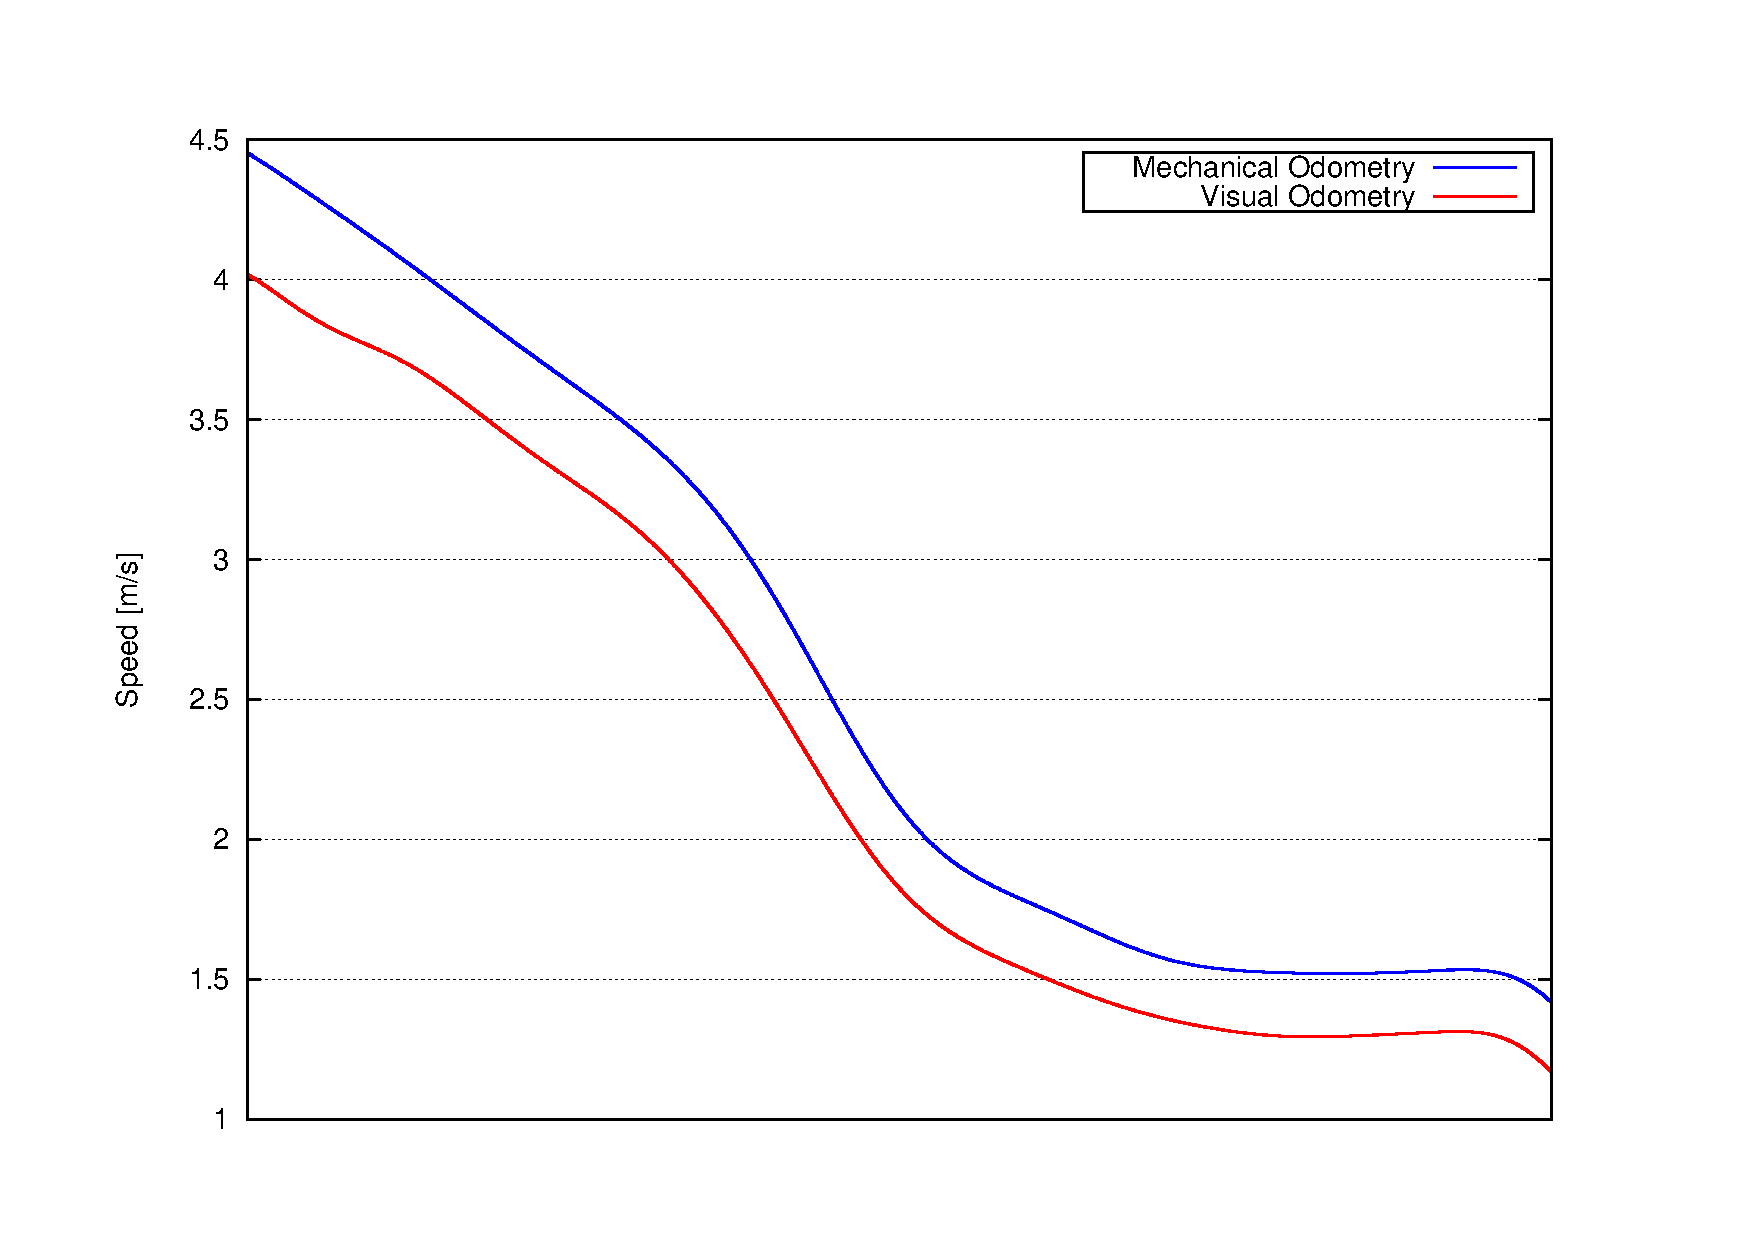
\includegraphics[trim=50 50 90 60, clip]{speed}
  \caption{Comparison between the speed values obtained through visual odometry compared to mechanical odometry.}\label{fig:cp05_ego_speed}
\end{figure}

\section{Detection}\label{ch:chapter05_02_03}
\todo{Si me sobra tiempo, intentar hacer un estudio más exhaustivo usando las imágenes de Daimler}
% Tasa de deteccion
\begin{figure*}[th]
        \centering
        \begin{subfigure}[b]{0.5\textwidth}
                \centering
                \includegraphics[width=\textwidth, trim=50 40 80 60,clip]{recall}\label{fig:cp05_recall}
                \caption{Recall}
                \label{fig:recallChart}
        \end{subfigure}%        
        ~ %add desired spacing between images, e. g. ~, \quad, \qquad etc.
          %(or a blank line to force the subfigure onto a new line)
        \begin{subfigure}[b]{0.5\textwidth}
                \centering
                \includegraphics[width=\textwidth, trim=50 40 80 60,clip]{precision}\label{fig:cp05_precision}
                \caption{Precision}
                \label{fig:precisionChart}
        \end{subfigure}%
        
%         ~ %add desired spacing between images, e. g. ~, \quad, \qquad etc.
          %(or a blank line to force the subfigure onto a new line)
        \begin{subfigure}[b]{0.5\textwidth}
                \centering
                \includegraphics[width=\textwidth, trim=50 40 80 60,clip]{f1}\label{fig:cp05_f1}
                \caption{$F_1$}
                \label{fig:f1Chart}
        \end{subfigure}%
        ~ %add desired spacing between images, e. g. ~, \quad, \qquad etc.
          %(or a blank line to force the subfigure onto a new line)
        \begin{subfigure}[b]{0.5\textwidth}
                \centering
                \includegraphics[width=\textwidth, trim=50 40 80 60,clip]{similarity}\label{fig:cp05_similarity}
                \caption{Similarity}
                \label{fig:similarityChart}
        \end{subfigure}
        \caption{Detection rate obtained by our method, compared with our implementation of the method of \cite{danescu2012particle}.}\label{fig:cp05_detection_rate}
\end{figure*}

\section{Performance}\label{ch:chapter05_02_04}
% Relacion tiempo-particulas
\begin{figure}[th]
  \centering
  \includegraphics[trim=50 50 90 60, clip]{timesVsParticles}
  \caption{Comparison of the time needed for the each iteration when the number of particles increases.}\label{fig:cp05_time_vs_particles}
\end{figure}

% Decir los tiempos en Hz (ya se dijo arriba, pero se puede repetir)
 
\section{Summary}\label{ch:chapter05_03}
 
% Decir que el código correspondiente a esta parte de la tesis se encuentra disponible en GITHUB
% Decir que se puede ver un video en youtube con los resultados
% Ventajas:
% Rápido
% repetir las ventaja de danescu
% Mejora el estado del arte si lo comparamos con Danescu
% - 3d completo
% - Permitimos movimiento en las 3 dimensiones
% - Otras ventajas q se me ocurran haciendo la parte de resultados
% 
% Trabajo futuro:
% Incluir informacion de color
% Hacer seguimiento a lo largo del tiempo de los obstaculos para poder aplicar filtro de kalman
% Mejorar mecanismo de segmentacion
% Implementar version paralela q haga uso de las ventajas de un grid
 
 
 
 
\acresetall

% %%
%%  chapter00.tex - Obstacle Detection and Planning for Autonomous Vehicles based on Computer Vision Techniques
%%
%%  Copyright 2014 Néstor Morales <nestor@isaatc.ull.es>
%%
%%  This work is licensed under a Creative Commons Attribution 4.0 International License.
%%

\addchap{Conclusions}

In this thesis, four different object detection tracking approaches, two methods for global and local path planning and a evaluation of two state-of-the-art algorithms with different configurations have been presented. Based on this, the goal of this thesis, the study of computer vision methods for obstacle detection and their avoidance for the Verdino prototype, is achieved.

The first of these approaches was based on the generation of a database in which each image had geographical information associated. In real time, the vehicle captured images from the onboard images and those were compared with the nearest image in the database by using classical image registration techniques. The changes detected were the obstacles in the way of the vehicle. 

With this approach, we evaluated the influence of the distance and angle difference between the compared images to the quality of the results. Conclusions were that the method works properly if distance is below 1\,m and the angle difference is below 10\textdegree. We also evaluated the influence of the illumination difference between images, concluding that the best results were obtained when this difference was below 20\%.

However, this approach has some limitations that can not be overcome using image registration techniques. First, we need a highly populated database if we want to be sure that we fulfill the distance and brightness difference limitations established. Also, as we are working with just an image of the camera, we can not locate the obstacles detected in real world coordinates. Finally, we know where the obstacles are, but we do not know were are they going to, so we need a tracking mechanism.

With these limitations in mind, we decided to isolate the last problem and develop a method for the tracking of generic obstacles without the need of a model in scenes captured by static cameras. The peculiarity of this method is that we do not track the obstacles as a whole object but we detect the trajectory followed by each part of them independently, detecting the flow of their contour.

The method consisted on the segmentation of the foreground of the scene using some state-of-the-art methods, extracting the contour of the obstacles. This contour was tracked between frames using a non rigid point set registration method, getting a match between points of different frames. These matches, joined along the frames, formed the trajectories of the points.

With this method, we demonstrated that is was possible to do such a tracking by using just geometrical information. Also, we evaluated the behavior of four different foreground segmentation methods (\cite{lopez2011stochastic, lopez2011foreground, guo2011hierarchical, reddy2012improved}), demonstrating that that from \cite{reddy2012improved} was the one that fulfilled the most our needs. Same was done for the six non rigid point set registration methods, of which the Coherent Point Drift was the one that gave the best results. Also, we compared our method with a simple optical flow tracker and a Kinect based method, showing that our method gave better results in certain circumstances.

However, the method is still not enough for our goal. It depends on static cameras, while we want to use the tracker with the images captured by the onboard cameras. Because of that, we started exploring some 3D reconstruction algorithms, and we found different approaches. Most of them were based on dense reconstruction, while some of them did a simplification of the reconstructed world by assuming certain conditions.

Inside the dense reconstruction methods, there were many different algorithms, making the choice difficult. One of the contributions of this thesis is the development of a automatized framework for the evaluation of dense reconstruction algorithms. This framework allows testing the algorithms using long sequences, at different weather and illumination conditions. This solved the problem existing for other previous evaluations in which the testing images were taken in laboratories, under controlled conditions; or in which sequences were too short with a ground truth edited by hand.

In these evaluation tests, we found some interesting results. We concluded that the use of filtering strategies reduces the number of wrong pixels and enhances the accuracy of the results. About the strategies used for the evaluation of the algorithms, we demonstrated that it is possible to do such statistics without the need of a \ac{LIDAR}-based ground truth (which despite of the great reliability of the statistics obtained with it, it is quite expensive in terms of the required equipment and the time needed for the post-processing of the captured data). The use of a prior on the vehicle movement was successfully exploited to identify a portion of the wrongly reconstructed points, making it suitable for the evaluation of big data-sets, thus covering a broad range of environmental conditions. In the other hand, the use of a third camera for evaluation looks feasible, but in practice the obtained results were not very discriminative.

We also explored other alternatives to dense reconstruction. Starting from the works in \cite{benenson2011stixels} and \cite{gunyel2012stixels}, we successfully developed a method for obstacle detection and tracking based on the stixels world described in \cite{badino2009stixel}. With this work, we shown that the use of a two-level tracking allows outperforming the existing methods about tracking in this field. Also the use of the Hellinger distance improved the tracking results. Apart from that, we also shown that, if speed is preferred over accuracy, object based tracking is possible, in which objects are obtained through a simple clustering method and then are tracked by using the illumination information between the obstacles.

Going back to the dense reconstruction methods, we also developed a tracking method able to receive a point cloud as input and detect the objects and their movement direction and speed, based just on their position in real world coordinates and a particle filter. Although we centered this work on dense stereo reconstruction based point clouds, it is also able to work with point clouds provided by other sensors, like for example \acp{LIDAR}, as we are not using color information. This is done thanks also to a modular implementation of the method. The use of a particle filter based approach allows avoiding complex probabilities-related calculations, and the use of a voxel grid allows working in three dimensions without increasing the complexity, as well as a more specific knowledge of the obstacle, which is not limited just to the more external boundaries of the obstacle through the use of cuboids.

Based on the detected obstacles, we developed a path planner scheme that allows the vehicle to reach a goal in the map while avoiding those objects. We divided this scheme into global and local planner. With the global planner, we shown a different strategy for the generation of trajectories based on \ac{MSVM}, in which each obstacle was a class, and the decision borders the possible paths, which were joined together with the use of a \acl{NNG} and a \acl{RNG}. This graph was updated with the new obstacles, avoiding to compute the whole graph again. The advantages of using this method as a base is that we can generate continuous non-linear border lines that allow the creation of smooth, short and safe paths. The use of the \ac{GPU} reduces the required computational time. 

About the local planner, we developed a method that, based on the Frenét space is able to generate smooth paths that allow, at the same time, following the trajectory and avoiding the obstacles in the way. Generation of the tentative paths is simplified as speed is out of the model of the tracks generation, so it is reduced to the computation of a set of parameters that define a third order polynomial. We also use different lateral offsets with respect to the global plan, so the avoidance of the obstacles is considered. Then, the use of a cost function allows selecting the best path.

With all these methods working, we put the best of them all together, showing that they were completely suitable for the application for which they were thought. We used our planner together with both the stixels world and the particle filter approaches. We observed that both were good enough to be used for obstacle detection and avoidance tasks, except from the limitations we already knew for them (i.e., the need of a planar ground for the stixels, or the assumption of a maximal speed between frames for the \ac{PF} based approach).

\addsec{Future Work}

However, there is still much work to do and many things that could be improved. 

\begin{itemize}
 \item We saw that one of the limitations of the method is the maximal distance and angle between the images. Because of that, we think that using other method for the matching of features between images is possible. In fact, we have done some tests in which we used the \ac{GPU} for the computation and matching of \ac{SURF} features (\cite{bay2008speeded}), in which the times obtained were suitable for such approach.
 \item This method could be used also for other tasks as the improvement of some of the existing change detection methods for aligned video sequences, like those presented by \cite{diego2011video, evangelidis2011slice, evangelidis2011efficient}.
 \item The output obtained for the non rigid contour tracking method described is still not being used at all. We think that this output could be used for many applications, not just related to \ac{ADAS}, but also to motion analysis in videos or \ac{HMI} systems.
 \item We would like to go beyond the use of static bidimensional image sequences, and extend the method to 3D. A way to do that would the segmentation of a disparity map, in which the contours used would be the borders of the segmented regions. Then, these could be easily transformed to real world coordinates.
 \item Another way to do that would be through the addition of new dimensions to the points used in the non-rigid point set registration step. Despite the Coherent Point Drift algorithm allows doing that, it would require the optimization of the current implementation we are using of this method. This will also allow including color information easily. We started a \ac{CUDA} based implementation of this method, with promising results.
 \item Despite the method used in the results section for the evaluation of this tracking method is reset each frame, we would like to extend it in order to use it for the analysis of the movement of an object. This would require to generate a model of the tracked object, but the analysis of its movement could be done through this method.
 \item About the evaluation of the dense reconstruction methods, the use of a third camera was promising, but results were not as good as expected. In the future, we expect to use different metrics to measure the similarity between the control camera and virtual images. Also more experiments could be performed, including sequences with different atmospheric conditions like other hours in a day.
 \item We also want to try new methods for stixels computation. A possibility would be using the polar rectification for the combination of tracking and reconstruction in a single process. 
 \item We could use the tracking output as a clue for the clustering process, in which we just use the stixels for which a correspondence is found for the clustering process.
 \item The particle filter based approach is using just position information for the tracking of the obstacles. We think that results would be improved if color information is used. This will avoid the use of sensors different from stereo cameras, but we could think on an schema in which several sensors are joined, being a stereo pair one of them.
 \item We also would like to track the trajectories of the obstacles along the sequences, which is not being done right now.
 \item We also want to do a parallel implementation of the method, which should be easy to perform and will give better results in term of time used.
 \item Regarding to the path planning methods, there also some work that could be done. For example, new clustering strategies could be applied for the global planner.
 \item Also, the use of \ac{MSVM} could be combined with other classical approaches.
 \item New cost of long-term control strategies could be applied for the generation and selection of the candidate paths in the local planner.
 \item The final selection of the applied steering angle and speed could be improved. Some approaches we have considered are the use of a \ac{PID} controller or even more complex control strategies, as a predictive controller.
\end{itemize}

Finally, with all these systems working, it would be interesting to do a more tight combination of them in which, based on the tracked obstacles, Verdino will be able to predict the future motion of the obstacles, giving it a behavior quite close to that followed by humans.

And then, maybe humans will not have to drive.

% \appendix
% \input{appendixA}
%\input{apendiceB}

\backmatter
\bibliography{references}

\end{document}
